%% LaTeX-Beamer template for KIT design
%% by Erik Burger, Christian Hammer
%% title picture by Klaus Krogmann
%%
%% version 2.1
%%
%% mostly compatible to KIT corporate design v2.0
%% http://intranet.kit.edu/gestaltungsrichtlinien.php
%%
%% Problems, bugs and comments to
%% burger@kit.edu

\documentclass[18pt]{beamer}

%% SLIDE FORMAT

% use 'beamerthemekit' for standard 4:3 ratio
% for widescreen slides (16:9), use 'beamerthemekitwide'

\usepackage{templates/beamerthemekit}
% \usepackage{templates/beamerthemekitwide}

\usepackage{graphicx}

%% TITLE PICTURE

% if a custom picture is to be used on the title page, copy it into the 'logos'
% directory, in the line below, replace 'mypicture' with the
% filename (without extension) and uncomment the following line
% (picture proportions: 63 : 20 for standard, 169 : 40 for wide
% *.eps format if you use latex+dvips+ps2pdf,
% *.jpg/*.png/*.pdf if you use pdflatex)

\titleimage{labor}

%% TITLE LOGO

% for a custom logo on the front page, copy your file into the 'logos'
% directory, insert the filename in the line below and uncomment it

\titlelogo{title}

% (*.eps format if you use latex+dvips+ps2pdf,
% *.jpg/*.png/*.pdf if you use pdflatex)

%% TikZ INTEGRATION

% use these packages for PCM symbols and UML classes
% \usepackage{templates/tikzkit}
% \usepackage{templates/tikzuml}

% the presentation starts here

\title[TruffleHog \& spp\_profinet]{TruffleHog \& spp\_profinet}
%\subtitle{2015}
\author{Maximilian Diez, Mark Giraud, Jan Hermes}

\institute{Fraunhofer IOSB}

% Bibliography

%\usepackage[citestyle=authoryear,bibstyle=numeric,hyperref,backend=biber]{biblatex}
%\addbibresource{templates/example.bib}
%\bibhang1em

\begin{document}

% change the following line to "ngerman" for German style date and logos
\selectlanguage{ngerman}

%title page
\begin{frame}
\titlepage
\end{frame}

%table of contents
%\begin{frame}{Gliederung}
%\tableofcontents
%\end{frame}

\section{Einleitung}

\begin{frame}
    \begin{itemize}
      \item PROFINET zur einfacheren Vernetzung von Industrieanlagen
      \pause
      \item Sicherheit?
      \pause
      \item Paketanalyse mit Snort
      \pause
      \item ----
    \end{itemize}
\end{frame}
\begin{frame}
\begin{figure}
	\centering
	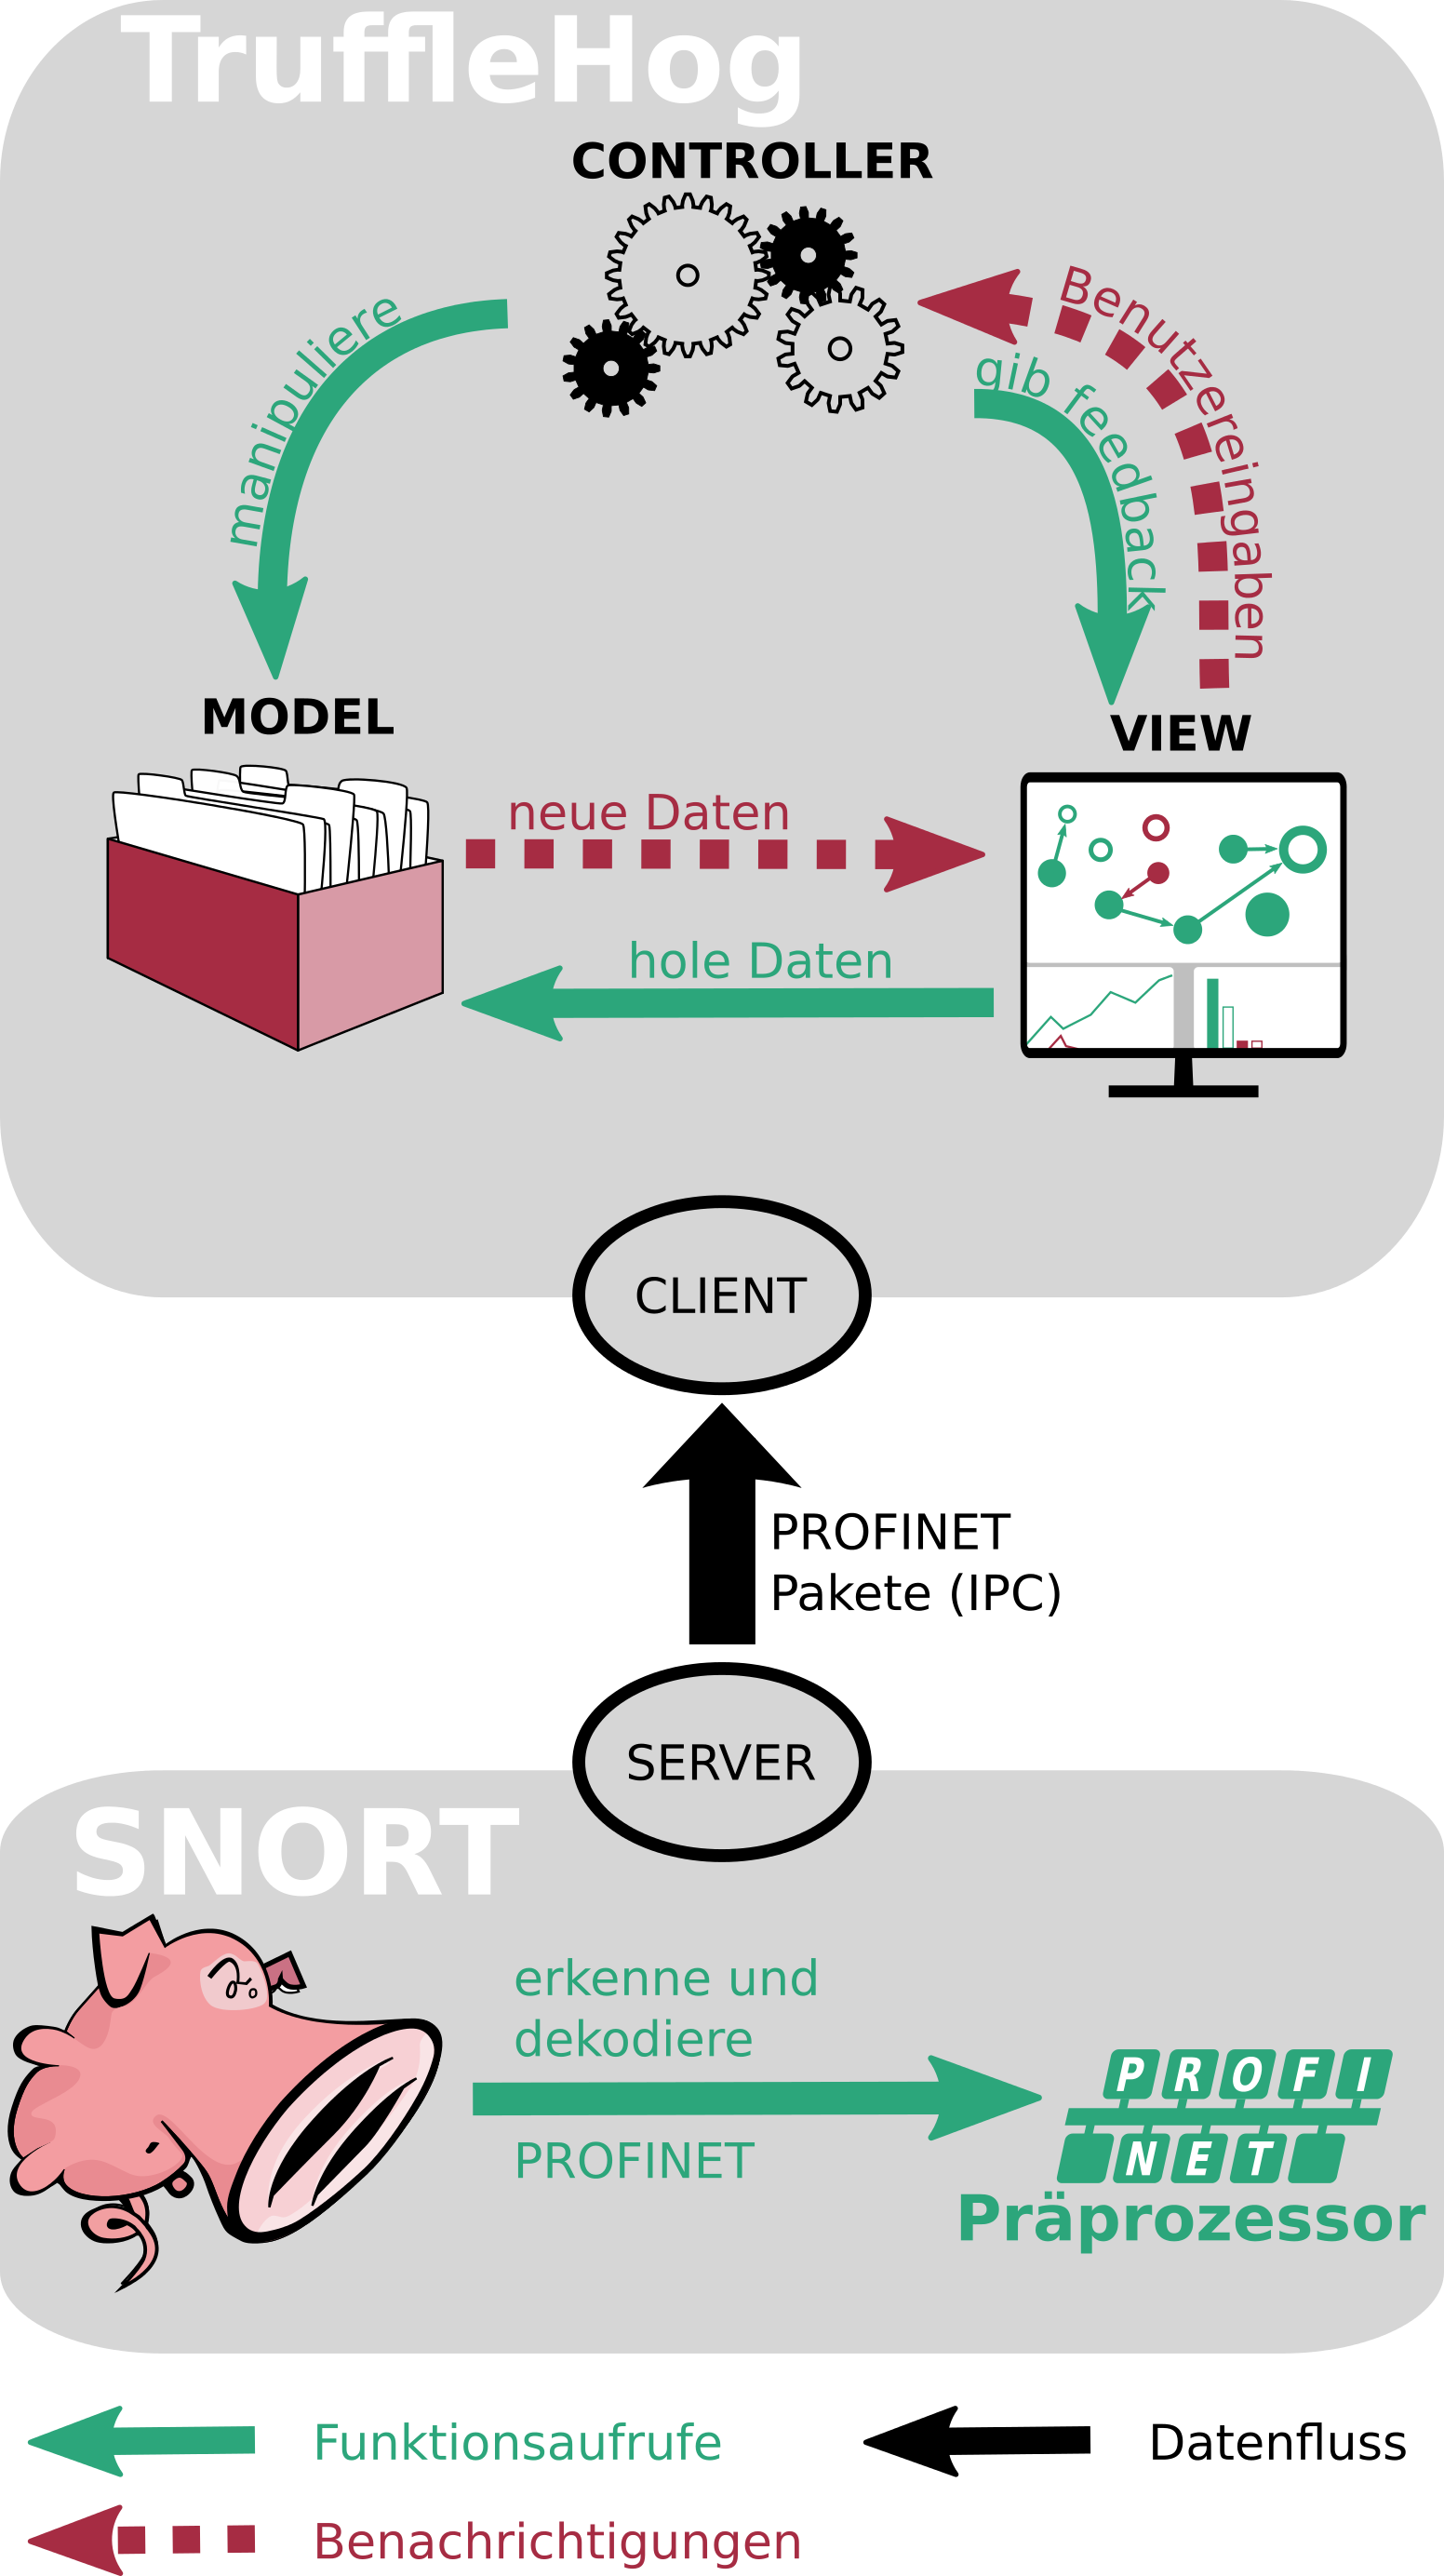
\includegraphics[height=0.9\textheight]{./images/intro_diagram.png}
\end{figure}
\end{frame}



\appendix
\beginbackup

%\begin{frame}[allowframebreaks]{References}
%\printbibliography
%\end{frame}

\backupend

\end{document}
